% -*- program: xelatex -*-
%\documentclass[12pt, compress]{beamer} 
\documentclass[12pt, compress]{beamer}       
%\documentclass[notes=only]{beamer}

\usepackage{fontspec}
	
\setsansfont{PT Sans}
\setmonofont{Liberation Mono}

\usepackage{beamerthemesplit}
\usefonttheme[onlymath]{serif}
%\DeclareFontEncoding{T1}
\fontencoding{T1}

%\usepackage[T2A]{fontenc} 
%\usepackage[utf8x]{inputenc}
\usepackage[russian]{babel}
\usepackage{listings}

\usepackage{amsmath,amssymb,amsthm} 
\hypersetup{unicode=true}
\usepackage{graphics,graphicx}
\usepackage{verbatim} 
\usepackage{fancyvrb}
\usepackage{booktabs}
\usepackage{media9}
\usepackage[super]{natbib}
\usepackage{color}
\definecolor{mygreen}{RGB}{28,172,0} % color values Red, Green, Blue
\definecolor{mylilas}{RGB}{170,55,241}
\definecolor{codecolor}{RGB}{0,120,0}
\definecolor{light-gray}{gray}{0.95}
\definecolor{light-green}{rgb}{0.93, 1, 0.8}
\definecolor{light-yellow}{rgb}{1,1,0.85}
\definecolor{dark-blue}{rgb}{0,0,0.6}
\definecolor{dark-red}{rgb}{0.7,0,0.0}
\definecolor{dark-green}{RGB}{10,150,0}

\usepackage{pifont}% http://ctan.org/pkg/pifont
\newcommand{\cmark}{\textcolor{green}{\ding{51}}}
\newcommand{\xmark}{\textcolor{red}{\ding{55}}}

\setbeamercolor{frametitle}{fg=dark-red,bg=gray!10}
\setbeamerfont{title}{series=\bfseries,parent=structure}
\setbeamerfont{frametitle}{series=\bfseries,parent=structure}

\setbeamertemplate{blocks}[rounded][shadow=false]
\setbeamertemplate{navigation symbols}{}

\newcommand{\code}[1]{\textcolor{dark-green}{\texttt{#1}}}
\newcommand{\cleartitlepage}[1]{\begin{frame}[plain]\begin{center}\textsc{#1}\end{center}\end{frame}}
\renewcommand{\emph}[1]{\textcolor{dark-blue}{#1}}
\newcommand{\emphb}[1]{\textcolor{dark-blue}{\textbf{#1}}}
\newcommand{\lstcomment}[1]{\textcolor{dark-green}{\# \texttt{#1}}}

\usepackage{dirtree}

\usetheme{CambridgeUS}
\usecolortheme{lily}

\lstset{basicstyle=\ttfamily,
    language=python,    
    keepspaces=true,
    extendedchars=\true,
    basicstyle={\small},
    breaklines=true,
    morekeywords={matlab2tikz},
    keywordstyle=\color{blue},
    morekeywords=[2]{1}, keywordstyle=[2]{\color{blue}},
    identifierstyle={ \bf \color{black} },
    stringstyle=\color{mylilas},
    commentstyle=\color{mygreen},%
    showstringspaces=false,
    numbers=left,%
    numberstyle={\scriptsize \color{gray}},
    numbersep=7pt, 
    emph=[1]{case,switch,otherwise,nonlocal,as,yield, with},emphstyle=[1]\color{blue}, 
    frame=single,    
    rulecolor=\color{red},    
    backgroundcolor=\color{light-gray},
    xleftmargin=0.3cm,
    frame=l,framesep=4pt,framerule=0.5pt,
    escapechar=|
    %lineskip=-1.0pt,
    %emph=[2]{word1,word2}, emphstyle=[2]{style},    
}

\usepackage{tikz}
\usetikzlibrary{positioning} 
\tikzset{cbutton/.style={rectangle,minimum width=10mm,thick,draw=red!50!black!50,
top color=white,bottom color=red!50!black!30}}
\tikzset{mbutton/.style={rectangle,minimum width=10mm,thick,draw=black!20,
top color=white,bottom color=black!30}}

\usetikzlibrary{arrows,shapes}
\tikzstyle{every picture}+=[remember picture]


\makeatother
\setbeamertemplate{footline}
{
  \leavevmode%
  \hbox{%  
  \begin{beamercolorbox}[wd=.3\paperwidth,ht=2.25ex,dp=1ex,center]{author in head/foot}%
    \usebeamerfont{author in head/foot}\insertshortauthor
  \end{beamercolorbox}%  
  \begin{beamercolorbox}[wd=.6\paperwidth,ht=2.25ex,dp=1ex,center]{title in head/foot}%
    \usebeamerfont{title in head/foot}\insertshorttitle
  \end{beamercolorbox}%
  \begin{beamercolorbox}[wd=.1\paperwidth,ht=2.25ex,dp=1ex,center]{date in head/foot}%
   %\insertframenumber{} / \inserttotalframenumber\hspace*{1ex}
    \insertframenumber{} 
  \end{beamercolorbox}}%
  \vskip0pt%
}

\setbeamertemplate{headline}{}
%\setbeamertemplate{footline}{}
 
\AtBeginSection[]{
  \begin{frame}[plain]
  %\vfill  
  \begin{tikzpicture}
  \useasboundingbox (0,0) rectangle(\the\paperwidth,\the\paperheight);  
  \fill[color=dark-red]   (-1cm, 3.9cm) rectangle(\the\paperwidth, 5.9cm);
  %\usebeamerfont{title}\insertsectionhead\par%
  %\node[text width=\the\paperwidth,align=center] at (current page.center) {\color{ExecusharesWhite}\Large\textbf{\insertsectionhead}};  
  \node[text width=\the\paperwidth,align=center] at (6cm,4.9cm) {\color{white}\Large\textbf{\insertsectionhead}};  
  \end{tikzpicture}
  \end{frame}
}



% ============================================================================

\title[Inkscape]{Inkscape}
\subtitle{(Компьютерная графика)}
\author[Самарский университет]{Юдинцев В. В.}
\institute{Кафедра теоретической механики\\Самарский университет}
\date{\today}

\usepackage{tikz}
\usetikzlibrary{positioning} 
\tikzset{cbutton/.style={rectangle,minimum width=10mm,thick,draw=red!50!black!50,
top color=white,bottom color=red!50!black!30}}
\tikzset{mbutton/.style={rectangle,minimum width=10mm,thick,draw=black!20,
top color=white,bottom color=black!30}}


\tikzstyle{block} = [rectangle, draw, fill=yellow!20, text width=5em, text centered, rounded corners, minimum height=5em]
\tikzstyle{subblock} = [rectangle, draw, fill=white, text width=2em, text centered, minimum height=1em]
\tikzstyle{module} = [rectangle, draw, fill=none, text width=5em, text centered, rounded corners, minimum height=5em]
\tikzstyle{line} = [draw, ->]

\usepackage{menukeys}

\begin{document}

{
\setbeamercolor{background canvas}{bg=white} 
\usebackgroundtemplate{\includegraphics[width=17cm,height=\paperheight]{sputnik.png}}
\begin{frame}[plain]
%\begin{figure}[h]
%  \centering
  %\includegraphics[width=0.3\textwidth]{}
%\end{figure}
\maketitle
\end{frame}
}

%
% \frame{\frametitle{Содержание}\tableofcontents}
%

\begin{frame}[c]
\frametitle{Цель курса ``Компьютерная графика''}
Освоение инструментов (компьютерных программ) для создания качественных \emph{технических иллюстраций}.
\end{frame}

\begin{frame}
\frametitle{Плохой пример}
\includegraphics[width=1\textwidth]{плагиат.png}
\end{frame}

\begin{frame}
\frametitle{Техническая иллюстрация}
\emph{Техническая иллюстрация} -- иллюстрация, цель которой научно и с достаточной документальной точностью наглядно изобразить тот объект, на который указывает автор текста.

\vspace{10pt}

\emph{Техническая иллюстрация} решает информационную, а не художественную задачу. 

\vspace{10pt}

К иллюстрациям относятся графические инструкции, графики, чертежи, изображения механических устройств, архитектурные изображения, изображения биологических видов, анатомические рисунки.
\end{frame}

\begin{frame}
\frametitle{Техническая иллюстрация}
\begin{figure}[htbp]
  \centering
  \includegraphics[width=0.95\textwidth]{PMS.png}
\end{figure}
\end{frame}

\section{Свободное ПО} 

\begin{frame}
\frametitle{Коммерческое ПО}
\emph{Система}
\begin{itemize}
  \item Microsoft Windows
\end{itemize}  
\emph{Офис}
\begin{itemize}
  \item MS Word / Excel
\end{itemize}  
\emph{Графика}
\begin{itemize}
  \item MS Word, MS Paint  
  \item Photoshop, CorelDraw
\end{itemize}
\emph{Прикладные программы (механика, математика)}
\begin{itemize}    
  \item MathCad 
  \item Mathematica
  \item MATLAB
  \item MSC.ADAMS/NASTRAN, ANSYS 
\end{itemize}  
\end{frame}

\begin{frame}
\frametitle{Свободное ПО}
\emph{Система}
\begin{itemize}
  \item Linux (Ubintu, Debian, Mint, elementary, Fedora, ...)
\end{itemize}  
\emph{Офис}
\begin{itemize}
  \item OpenOffice
  \item LaTeX
\end{itemize}  
\emph{Графика}
\begin{itemize}  
  \item Inkspace
  \item GIMP
\end{itemize}    
\emph{Прикладные программы}
\begin{itemize}  
  \item Python (numpy, scipy), SageMath
  \item OCTAVE (аналог MATLAB)
  \item R
\end{itemize}  
\end{frame}

\begin{frame}
\frametitle{Типы программного обеспечения}
\begin{columns}
\column{0.5\linewidth}
\begin{itemize}  
  \item \alert<+> {Свободное}
  \item \alert<+> {Бесплатное (freeware)}
  \item \alert<+> {Условно-бесплатное (shareware)}
  \item \alert<+> {Коммерческое}
  \item \alert<+> {Собственническое}  

\end{itemize}  
\column{0.5\linewidth}
\only<1>{\emph{Свободное программное обеспечение} -- программное обеспечение, пользователи которого имеют права на его неограниченную установку, запуск, свободное использование, изучение, распространение и изменение (совершенствование), а также распространение копий и результатов изменения.}
\only<2>{\emph{Бесплатное программное обеспечение} обеспечение не требует каких-либо выплат правообладателю. Бесплатное программное обеспечение обычно распространяется в бинарном виде, без исходных кодов и является проприетарным программным обеспечением.}
\only<3>{\emph{Условное бесплатное} программное обеспечение предлагает пользователю ознакомится с функциями программы до её покупки. Программа может быть ограничена по возможностям: сроку действия, функциональности.} 
\only<4>{\emph{Коммерческое} программное обеспечение -- программное обеспечение, распространяемое с целью получения прибыли.}
\only<5>{\emph{Собственническое} или проприетарное программное являеься частной собственностью авторов или правообладателей и не удовлетворяющее критериям свободного ПО. Правообладатель сохраняет за собой монополию на его использование, копирование и модификацию, полностью или в существенных моментах.}
\end{columns}
\end{frame}

\begin{frame}[t] 
\frametitle{Программа курса}
\begin{itemize}
  \item \emph{Inkscape} \\ 
  создания технических иллюстраций. 
  \item \emph{Gnuplot} \\   
  свободная программа для создания графиков. 
  \item \emph{Blender 3D} \\
  3D графика, построение анимации по результатам расчётов.
  \item \emph{Python (scipy/numpy)} \\ 
  интегрирование дифференциальных уравнения, построение графиков, экспорт результатов.
  \item \emph{Imagemagic, ffmpeg} \\   
  свободный набор утилит командной строки для обработки изображений и видеофайлов.
\end{itemize}
\end{frame}

\begin{frame}[c]
\frametitle{Философия Unix}
\begin{itemize}
  \item Пишите программы, которые делают что-то одно и делают это хорошо.
  \item Пишите программы, которые бы работали вместе.
  \item Пишите программы, которые бы поддерживали текстовые потоки, поскольку это универсальный интерфейс.   
\end{itemize}        
\end{frame}

\begin{frame}[t]
\frametitle{Философия Unix}
\begin{figure}[htbp]  
  \includegraphics[width=0.8\textwidth]{not_unix_way1.png}
\end{figure}
\end{frame}

\begin{frame}[t]
\frametitle{Философия Unix}
\begin{figure}[htbp]  
  \includegraphics[width=0.8\textwidth]{not_unix_way2.png}
\end{figure}
\end{frame}

\begin{frame}[t] 
\frametitle{Философия Unix}
\begin{figure}[htbp]  
  \includegraphics[width=0.8\textwidth]{unixway.png}
\end{figure}
\end{frame}

\begin{frame}[c] 
\frametitle{Анализ движения КА ``Аист-2'' и ``Ломоносов''}
\begin{figure}[htbp]  
  \includegraphics[width=1\textwidth]{Aist.png}
\end{figure}
\end{frame}


\section{Inkscape}

\begin{frame}[c]
\frametitle{Inkscape}
\emph{Inkscape} (Инкскейп) -- графический редактор \emph{векторных} изображений формата \emph{SVG}.

\vspace{5pt}

Применение
\begin{itemize}
  \item презентации, логотипы, визитки, плакаты;
  \item техническая графика;
  \item веб-графика: баннеры, макеты сайтов, пиктограммы для приложений и кнопок сайтов, графика для игр.
\end{itemize}
Inkscape -- свободное ПО.
\end{frame}



\begin{frame}
\frametitle{Форматы файлов}
\begin{itemize}
  \item Импорт \\
  SVG, SVGZ, CGM, EMF, DXF, EPS, PostScript, PDF, \alert{AI} (9.0 и выше), \alert{CorelDRAW}, Dia, Sketch, PNG, TIFF, JPEG, XPM, GIF, BMP, WMF, WPG, GGR, ANI, ICO, CUR, PCX, PNM, RAS, TGA, WBMP, XBM, XPM, ANI.
  \item Экспорт \\
  \alert{PNG}, SVG, \alert{EPS}, PostScript, \alert{PDF}, Dia, \alert{AI}, Sketch, POV-Ray, \alert{LaTeX}, OpenDocument Draw, GPL, \alert{EMF}, POV, \alert{DXF}.
\end{itemize}
\end{frame}

\begin{frame}
\frametitle{Векторная графика}
В \emph{векторной графике} изображение строится на основе математического описания элементарных геометрических объектов: точек, линий, сплайнов, окружностей, многоугольников.
\begin{figure}[htbp]
  \centering
  \includegraphics[width=0.4\textwidth]{растр-вектор.png}
\end{figure}
\vspace{5pt}

\emph{Растровое изображение} представляет собой сетку (матрицу) точек разного цвета.
\end{frame}

\begin{frame}[t]
\frametitle{Inkscape}
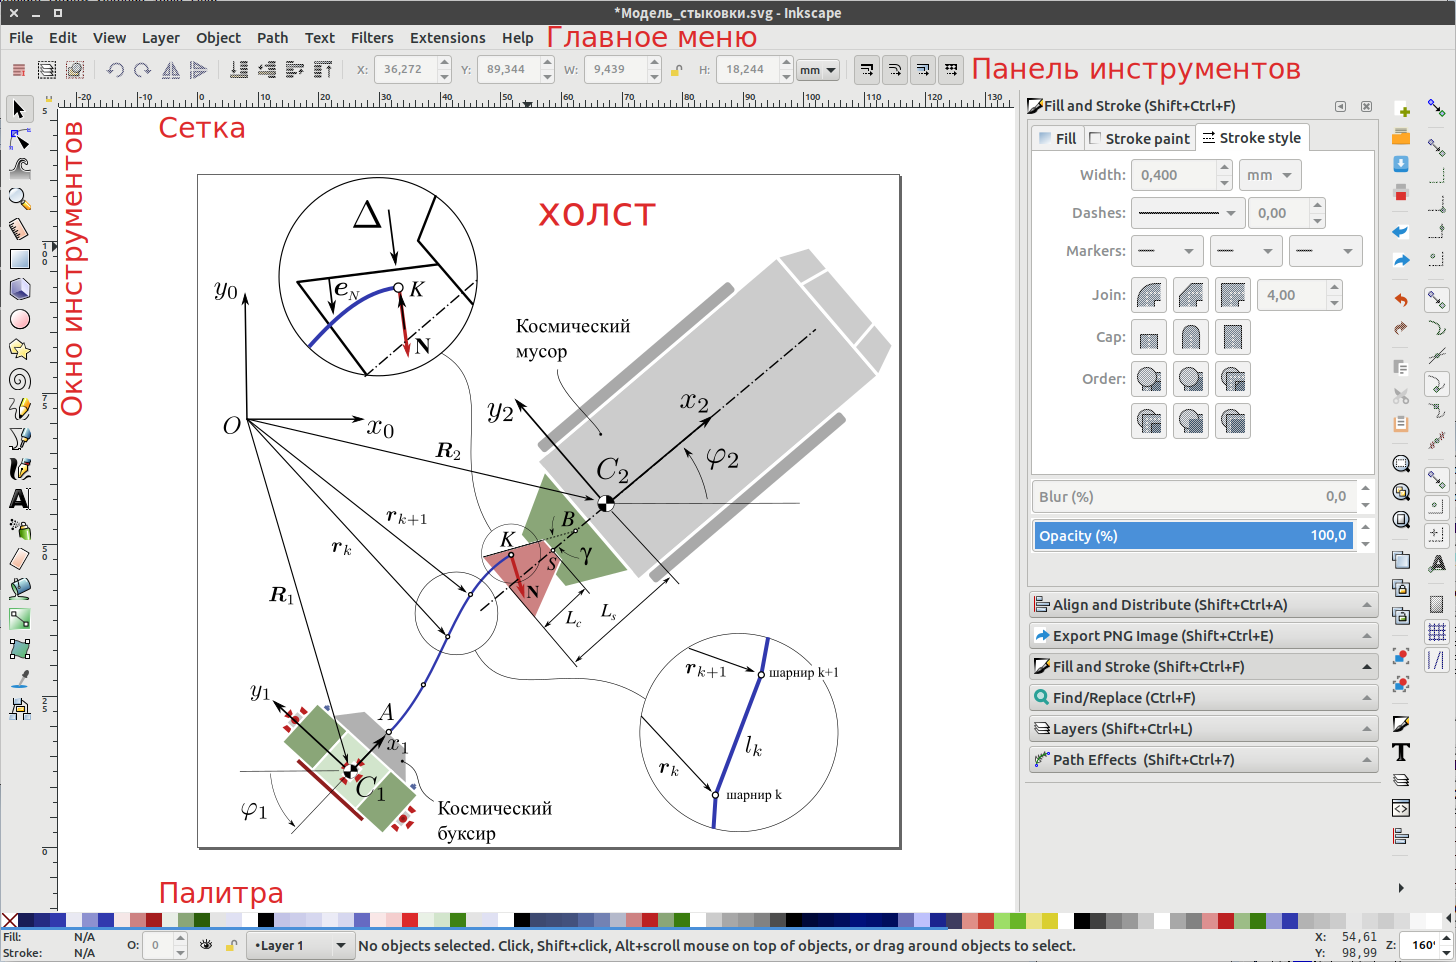
\includegraphics[width=1.0\textwidth]{inkscape1.png}
\end{frame}

\begin{frame}
\frametitle{Установка}
\url{https://inkscape.org/ru/}
\includegraphics[width=0.95\textwidth]{download.png}
\end{frame}


\begin{frame}[fragile]
\frametitle{Формат файла}
SVG (от англ. Scalable Vector Graphics — масштабируемая векторная графика) -- язык разметки масштабируемой векторной графики, предназначеный для описания двумерной векторной и смешанной векторно/растровой графики в формате XML.
\begin{lstlisting}
<svg>
<circle cx="102" cy="102" r="100" 
fill="rgb(234,234,234)" stroke-width="1" 
stroke="rgb(0,0,0)"/>
</svg>
\end{lstlisting}
SVG -- открытый стандарт.
\end{frame}

\begin{frame}[t]
\frametitle{Перемещение и масштабирование холста}
\begin{figure}[htbp]  
  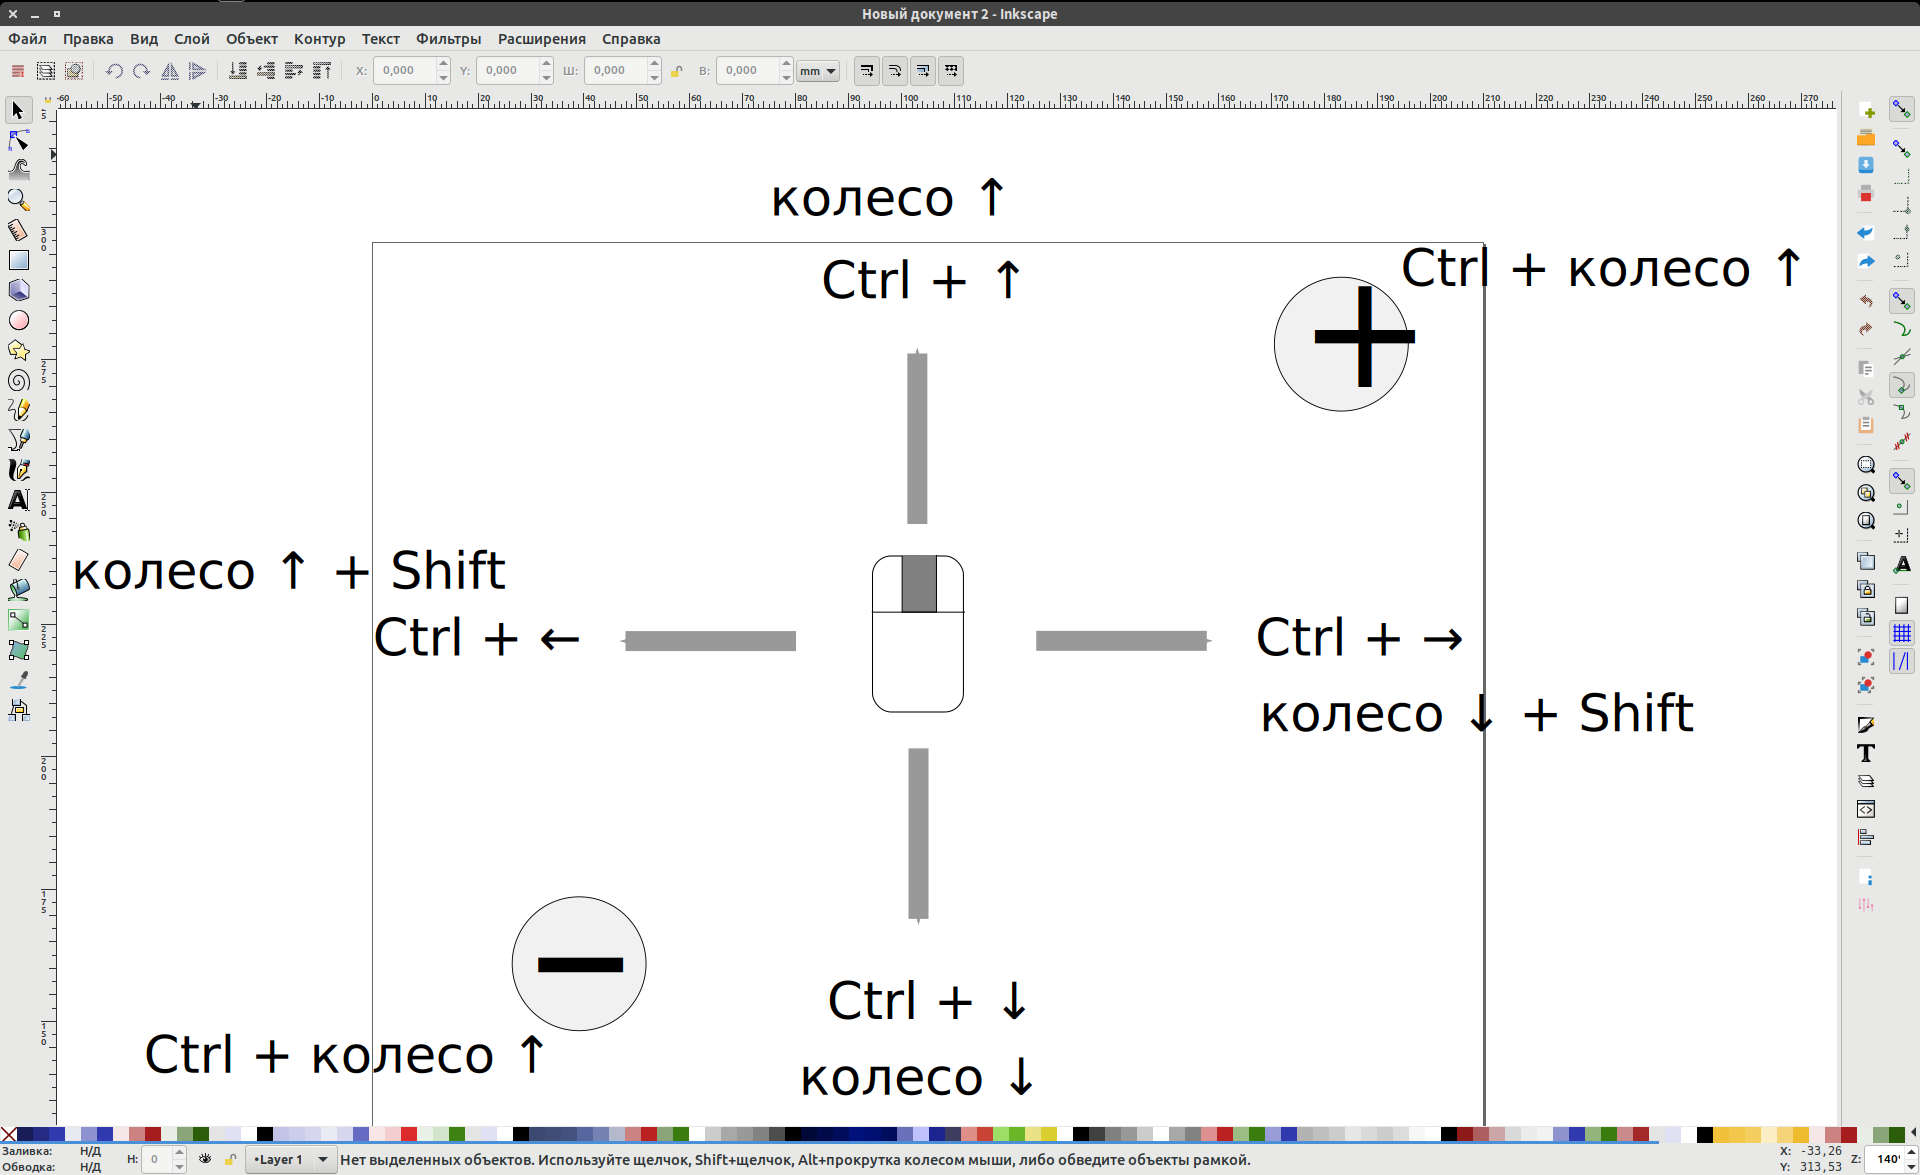
\includegraphics[width=1.0\textwidth]{pan_zoom.png}  
\end{figure}
\end{frame}

\begin{frame}[c]
\frametitle{Основные инструменты}
\begin{columns}
\column{0.6\linewidth}
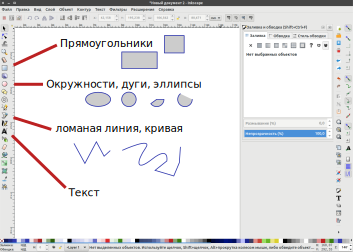
\includegraphics[trim={0 0 15cm 0},clip, width=0.9\linewidth]{Основные_инструменты.png}
\column{0.4\linewidth}
\begin{itemize}
  \item \keys{F4} прямоугольники
  \item \keys{F5} дуги и окружности 
  \item \keys{shift + F6} кривые/прямые 
  \item \keys{F8} текст
\end{itemize}
\end{columns}
\keys{ЛКМ} + перемещение
\end{frame}

\begin{frame}[c]
\frametitle{Перемещение, маштабирование, вращение}
Для выбора объекта, используется инструмент \emph{``Выделять и трансформировать''} -- \keys{F1} 

\includegraphics[width=0.25\textwidth]{масштаб.png}
\includegraphics[width=0.26\textwidth]{поворот.png}

Нажатие \keys{ctrl} ограничит перемещение вдоль горизонтальной или вертикальной оси, сделает маштабирование по ширине и высоте пропорциональным, а поворот -- с шагом 15 градусов.
\end{frame}

\begin{frame}
\frametitle{Перемещение, маштабирование, вращение}
\begin{center}
\includemedia[
  width=0.9\linewidth,height=0.6\linewidth,
  activate=pageopen,
  addresource=перемещение.mp4,
  flashvars={src=перемещение.mp4&autohide=1}
]{}{APlayer.swf} \\
\end{center}
\end{frame}

\begin{frame}
\frametitle{Порядок}
\begin{columns}
\column{0.6\linewidth}
\centering
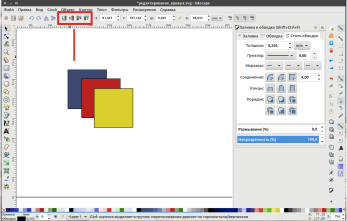
\includegraphics[trim={0 0 15cm 0},clip, width=0.95\textwidth]{порядок.png}
\column{0.4\linewidth}
\begin{itemize}
  \item \keys{Home} \\ на передний план
  \item \keys{PgUp} \\ на уровень вверх
  \item \keys{PgDn} \\ на уровень вниз
  \item \keys{End} \\ на задний план
\end{itemize}

\end{columns}
\end{frame}


\begin{frame}
\frametitle{Кривые \keys{shift + F6}}
\begin{columns}
\column{0.4\linewidth}
\centering
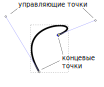
\includegraphics[width=1\textwidth]{безье.png}
\column{0.6\linewidth}
\begin{itemize}
  \item Одиночные нажатия \keys{ЛКМ} создают ломаную линию.
  \item Если после нажатия \keys{ЛКМ} начать перемещать мышь, не отпуская \keys{ЛКМ}, создаётся упраляющая точка для вершины.
  \item Управляющую точку можно создать после создания ломаной, выделив вершину \keys{ЛКМ} c нажатой клавишей \keys{shift}, и переместив курсор.
\end{itemize}
\end{columns}
\end{frame}

\begin{frame}
\frametitle{Свойства контура и заливка \keys{ctrl+F}}
\centering
\includegraphics[width=0.9\textwidth]{заливка.png}
\end{frame}

\begin{frame}
\frametitle{Свойства контура и заливка \keys{ctrl+F}}
\centering
\includegraphics[width=0.9\textwidth]{контур.png}
\end{frame}

\begin{frame}
\frametitle{Маркеры}
\centering
\includegraphics[width=0.9\textwidth]{контур-стрелка.png}
\end{frame}

\begin{frame}
\frametitle{Палитра}
\centering
\includegraphics[width=0.95\textwidth]{палитра.png}
\end{frame}

\begin{frame}
\frametitle{Редактирование кривых \keys{F2}}
\begin{center}
\includemedia[
  width=0.9\linewidth,height=0.6\linewidth,
  activate=pageopen,
  addresource=книга.mp4,
  flashvars={src=книга.mp4&autohide=1}
]{}{APlayer.swf} \\
\end{center}
\end{frame}

\begin{frame}
\frametitle{Сетка \keys{shift + \#}}
\begin{center}
\includemedia[
  width=0.9\linewidth,height=0.6\linewidth,
  activate=pageopen,
  addresource=сетка.mp4,
  flashvars={src=сетка.mp4&autohide=1}
]{}{APlayer.swf} \\
\end{center}
\end{frame}

\begin{frame}
\frametitle{Направляющие \keys{shift + |}}
\begin{columns}
\column{0.6\linewidth}
\includegraphics[width=1\textwidth]{направляющие.png}
\column{0.4\linewidth}
\only<1>{Для создания направляющих необходимо нажать \keys{ЛКМ} на горизонтальной или вертикальной линейке и переместить мышь вниз или вверх.}\only<2>{Направляющие перетаскиваются при помощи \keys{ЛКМ}. Для поворота направляющей необходимо нажать \keys{SHIFT}}\only<3>{Отображение направляющих управляется сочетанием \keys{SHIFT + |}}
\end{columns}
\end{frame}


\begin{frame}
\frametitle{Направляющие \keys{shift + |}}
\begin{center}
\includemedia[
  width=0.9\linewidth,height=0.6\linewidth,
  activate=pageopen,
  addresource=направляющие.mp4,
  flashvars={src=направляющие.mp4&autohide=1}
]{}{APlayer.swf} \\
\end{center}
\end{frame}




\section{Задание}

\begin{frame}
\frametitle{Задание 1}
\begin{itemize}
  \item Установить Inkscape \\
  \url{https://inkscape.org/ru/}
  \item Нарисовать механизм из задания для курсовой работы по теоретической механике.
\end{itemize}
\end{frame}


\end{document}
